%%
%% sample document for AAMAS'19 conference
%%
%% modified from sample-sigconf.tex
%%
%% see ACM instructions acmguide.pdf
%%
%% AAMAS-specific questions? F.A.Oliehoek@tudelft.nl
%%

\documentclass[sigconf]{aamas}  % do not change this line!

%% your usepackages here, for example:
\usepackage{booktabs}

%% your usepackages here, for example:
\usepackage{booktabs}

%% do not change the following lines
\setcopyright{ifaamas}  % do not change this line!
\acmDOI{doi}  % do noadat change this line!
\acmISBN{}  % do not change this line!
\acmConference[AAMAS'20]{Proc.\@ of the 19th International Conference on Autonomous Agents and Multiagent Systems (AAMAS 2020), B.~An, N.~Yorke-Smith, A.~El~Fallah~Seghrouchni, G.~Sukthankar (eds.)}{May 2020}{Auckland, New Zealand}  % do not change this line!
\acmYear{2020}  % do not change this line!
\copyrightyear{2020}  % do not change this line!
\acmPrice{}  % do not change this line!


%% the rest of your preamble here


%%%%%%%%%%%%%%%%%%%%%%%%%%%%%%%%%%%%%%%%%%%%%%%%%%%%%%%%%%%%%%%%%%%%%%%%%%%%%%%%%%%%%%%%%%%%%%%%%%%%%%%%%

\begin{document}

\title{Auctions for Allocation of Elastic Resources in Cloud Computing}  % put your title here!
%\titlenote{Produces the permission block, and copyright information}

% AAMAS: as appropriate, uncomment one subtitle line; check the CFP
%\subtitle{Extended Abstract}
%\subtitle{Industrial Applications Track}
%\subtitle{Socially Interactive Agents Track}
%\subtitle{Blue Sky Ideas Track}
%\subtitle{Engineering Multiagent Systems Track}
%\subtitle{Robotics Track}
%\subtitle{JAAMAS Track}
%\subtitle{Doctoral Mentoring Program}

%\subtitlenote{The full version of the author's guide is available as \texttt{acmart.pdf} document}


% AAMAS: submissions are anonymous for most tracks
\author{Paper \#XXX}  % put your paper number here!

%% example of author block for camera ready version of accepted papers: don't use for anonymous submissions
%
%\author{Ben Trovato}
%\authornote{Dr.~Trovato insisted his name be first.}
%\orcid{1234-5678-9012}
%\affiliation{%
%  \institution{Institute for Clarity in Documentation}
%  \streetaddress{P.O. Box 1212}
%  \city{Dublin} 
%  \state{Ohio} 
%  \postcode{43017-6221}
%}
%\email{trovato@corporation.com}
%
%\author{G.K.M. Tobin}
%\authornote{The secretary disavows any knowledge of this author's actions.}
%\affiliation{%
%  \institution{Institute for Clarity in Documentation}
%  \streetaddress{P.O. Box 1212}
%  \city{Dublin} 
%  \state{Ohio} 
%  \postcode{43017-6221}
%}
%\email{webmaster@marysville-ohio.com}
%
%\author{Lars Th{\o}rv{\"a}ld}
%\authornote{This author is the
%  one who did all the really hard work.}
%\affiliation{%
%  \institution{The Th{\o}rv{\"a}ld Group}
%  \streetaddress{1 Th{\o}rv{\"a}ld Circle}
%  \city{Hekla} 
%  \country{Iceland}}
%\email{larst@affiliation.org}
%
%\author{Valerie B\'eranger}
%\affiliation{%
%  \institution{Inria Paris-Rocquencourt}
%  \city{Rocquencourt}
%  \country{France}
%}
%\author{Aparna Patel} 
%\affiliation{%
% \institution{Rajiv Gandhi University}
% \streetaddress{Rono-Hills}
% \city{Doimukh} 
% \state{Arunachal Pradesh}
% \country{India}}
%\author{Huifen Chan}
%\affiliation{%
%  \institution{Tsinghua University}
%  \streetaddress{30 Shuangqing Rd}
%  \city{Haidian Qu} 
%  \state{Beijing Shi}
%  \country{China}
%}
%
%\author{Charles Palmer}
%\affiliation{%
%  \institution{Palmer Research Laboratories}
%  \streetaddress{8600 Datapoint Drive}
%  \city{San Antonio}
%  \state{Texas} 
%  \postcode{78229}}
%\email{cpalmer@prl.com}
%
%\author{John Smith}
%\affiliation{\institution{The Th{\o}rv{\"a}ld Group}}
%\email{jsmith@affiliation.org}
%
%\author{Julius P.~Kumquat}
%\affiliation{\institution{The Kumquat Consortium}}
%\email{jpkumquat@consortium.net}
%
%% The example's default list of authors is too long for headers
%\renewcommand{\shortauthors}{B. Trovato et al.}


\begin{abstract}  % put your abstract here!
Abstract goes here
\end{abstract}


% AAMAS: the ACM CCS are not needed within AAMAS papers
%%
%% The code below should be generated by the tool at
%% http://dl.acm.org/ccs.cfm
%% Please copy and paste the code instead of the example below. 
%%
%\begin{CCSXML}
%<ccs2012>
% <concept>
%  <concept_id>10010520.10010553.10010562</concept_id>
%  <concept_desc>Computer systems organization~Embedded systems</concept_desc>
%  <concept_significance>500</concept_significance>
% </concept>
% <concept>
%  <concept_id>10010520.10010575.10010755</concept_id>
%  <concept_desc>Computer systems organization~Redundancy</concept_desc>
%  <concept_significance>300</concept_significance>
% </concept>
% <concept>
%  <concept_id>10010520.10010553.10010554</concept_id>
%  <concept_desc>Computer systems organization~Robotics</concept_desc>
%  <concept_significance>100</concept_significance>
% </concept>
% <concept>
%  <concept_id>10003033.10003083.10003095</concept_id>
%  <concept_desc>Networks~Network reliability</concept_desc>
%  <concept_significance>100</concept_significance>
% </concept>
%</ccs2012>  
%\end{CCSXML}
%
%\ccsdesc[500]{Computer systems organization~Embedded systems}
%\ccsdesc[300]{Computer systems organization~Redundancy}
%\ccsdesc{Computer systems organization~Robotics}
%\ccsdesc[100]{Networks~Network reliability}


\keywords{Keywords here}  % put your semicolon-separated keywords here!

\maketitle

%% start of main body of paper

\section{Introduction}
\begin{itemize}
    \item Related works
    \item Resource allocation in cloud computing
    \item Market based allocation
    \item New Problem case
\end{itemize}

\section{System Model}
With the addition of a deadline with the job, this allows for the flexibility of the resources allocated by a server. Each job ($j$) has fixed resource requirements: storage ($s_j$), computation ($w_j$) and results data ($r_j$) with a deadline ($d_j$) and internal value ($v_j$). The server will allocation resources: loading speed ($s^{'}_j$), compute speed ($w^{'}_j$) and sending speed ($r^{'}_j$) so that the job deadline constraint holds (equation \ref{deadline_constraint}). \\

Optimisation
\begin{equation}
max \sum^J_j U_j (\sum^I_i x_{ij})
\end{equation}

Job Deadline constraint 
\begin{align} \label{deadline_constraint}
    \frac{S_j}{s_j} + \frac{W_j}{w_j} + \frac{R_j}{r_j} \leq D_j && \forall i = 1,\dots,I; j = 1,\dots,J
\end{align}

Jobs servers allocations
\begin{align}
    \sum^I_i x_{ij} \leq 1 && \forall j = 1,\dots,J
\end{align}

Server resource constraints
\begin{align}
    \sum^J_j S_j x_{ij} \leq S_i && \forall i = 1,\dots,I \\
    \sum^J_j w_j x_{ij} \leq W_i && \forall i = 1,\dots,I \\
    \sum^J_j (r_j + s_j) x_{ij} \leq R_i && \forall i = 1,\dots,I 
\end{align}

\section{Resource Allocation Auctions}
\subsection{Greedy Mechanism}
\begin{itemize}
    \item Possible greedy mechanisms
    \item Lower bound proof
    
\end{itemize}
\subsection{Decentralised Iterative Auction Mechanism}
The addition of the deadline constraint allows for cooperation between players to be incentived as to balance the requests for resources allowing more jobs to be allocated or for a small price. Following the VCG mechanism, we develop an auction where job prices are calculate on an individual server bases with the price being the difference in revenue when the job runs. 

If we find the value of an allocation where a job must be included and the value of the job not included then the difference is the value of the job on the server, to increase the price we add $\epsilon$. 
\begin{equation}
    Job price = V(\theta_J) - V(\theta^k_J) + \epsilon
\end{equation}

Each server solves the linear programming below that is the same as the problem case except with the server resource constraints modified to include the new job (k) without the allocation variable. 
\begin{align}
    \sum^J_j S_j x_{ij} + S_k \leq S_i && \forall i = 1,\dots,I; j = 1,\dots,J \\
    \sum^J_j w_j x_{ij} + w_k \leq S_i && \forall i = 1,\dots,I; j = 1,\dots,J \\
    \sum^J_j (r_j + s_j) x_{ij} + (r_k + s_k) \leq S_i && \forall i = 1,\dots,I; j = 1,\dots,J
\end{align}

\section{Empirical Evaluation}
\begin{figure*}
    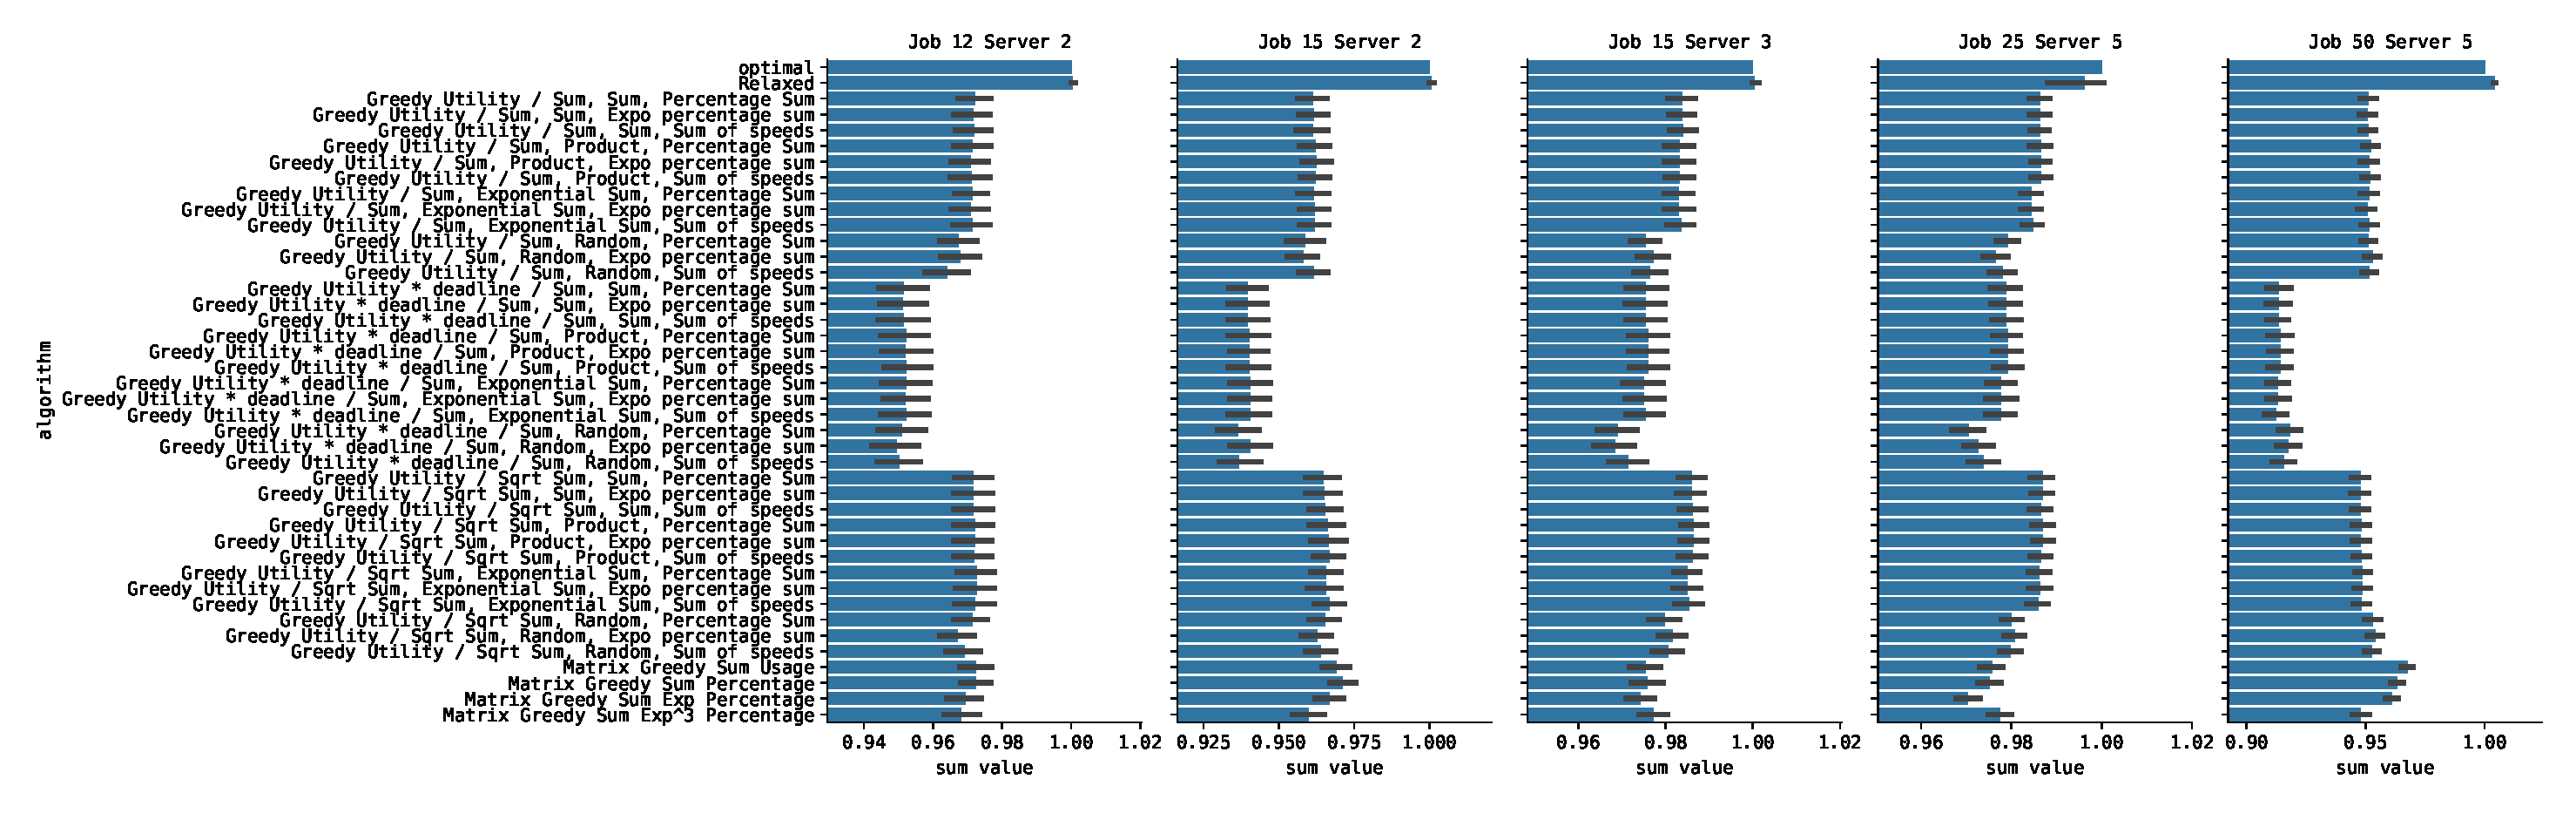
\includegraphics[width=\linewidth]{figures/greedy_basic_sum_value.eps}
    \caption{Greedy algorithms with basic model measuring the sum of values}
\end{figure*}
\begin{figure*}
    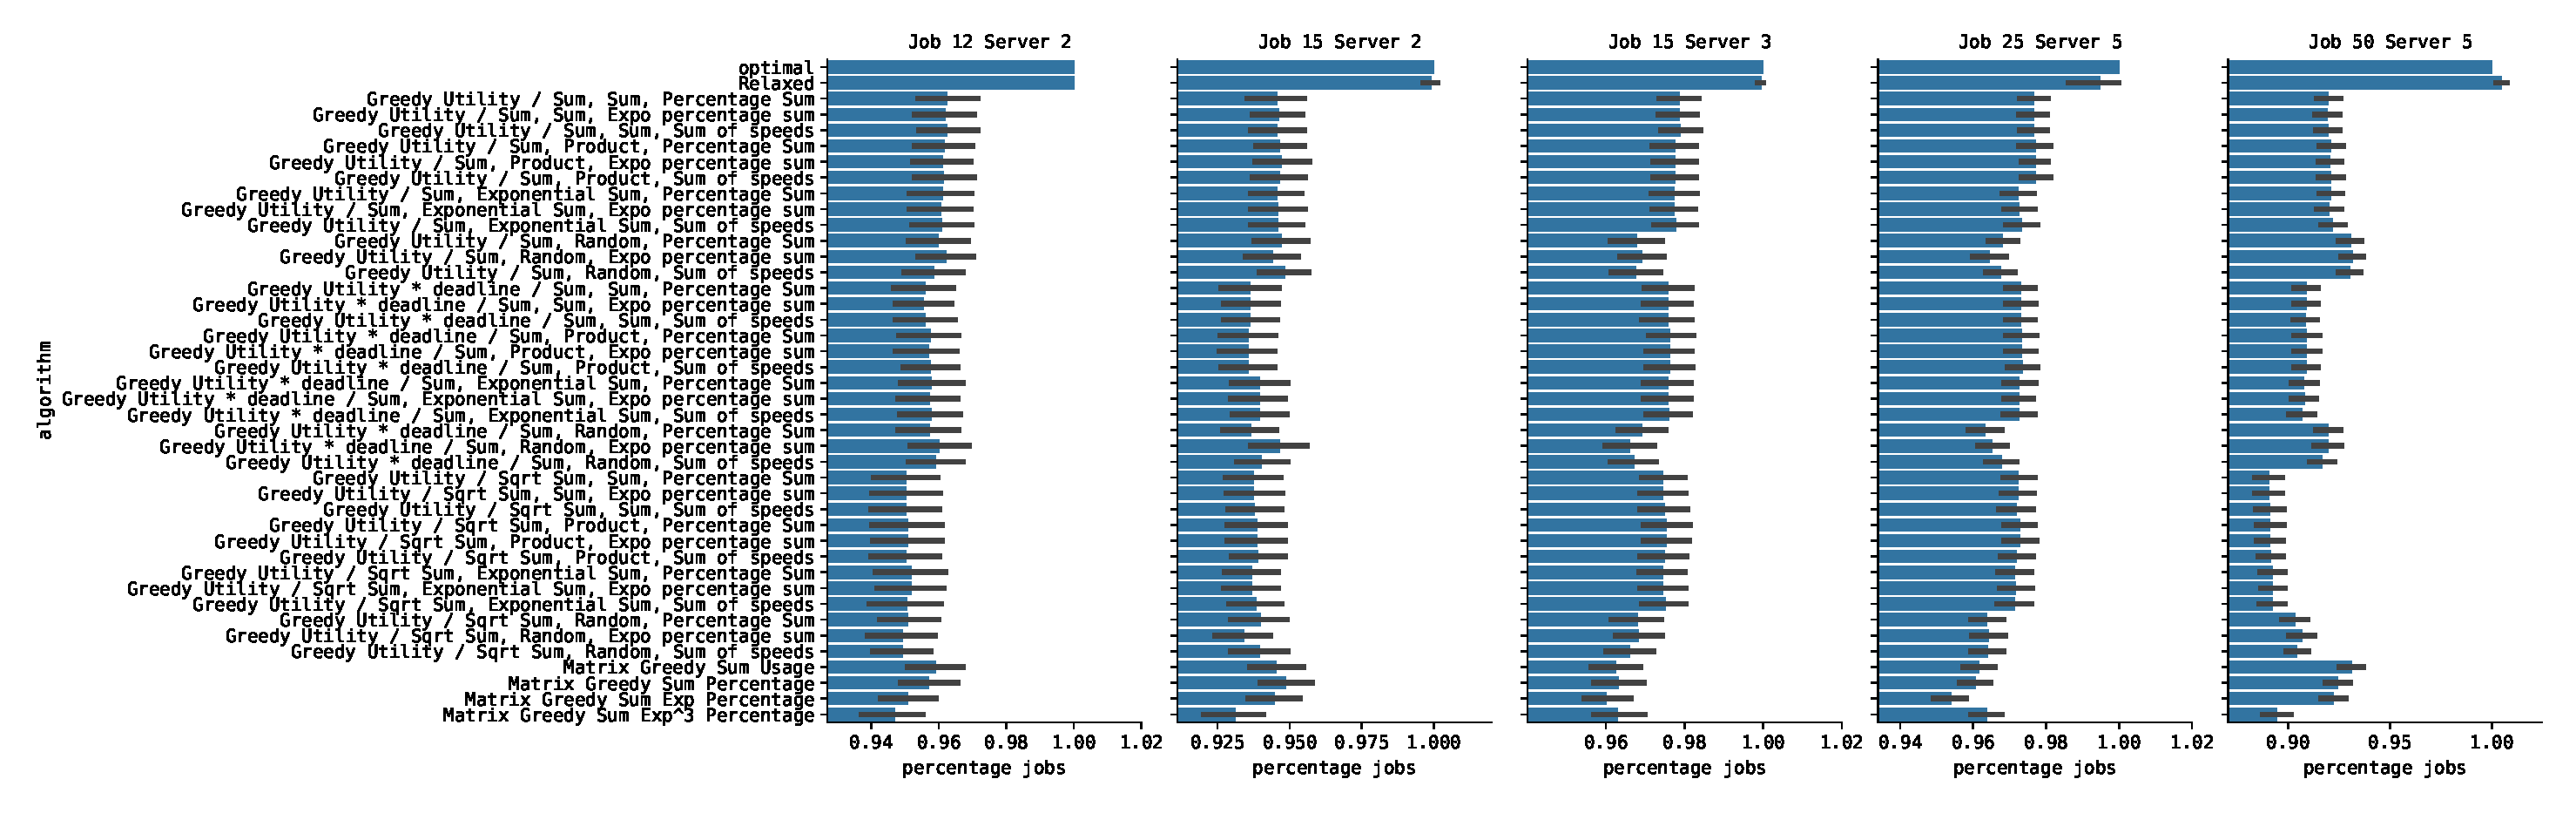
\includegraphics[width=\linewidth]{figures/greedy_basic_percentage_jobs.eps}
    \caption{Greedy algorithms with basic model measuring the percentage of jobs allocated}
\end{figure*}
\begin{figure*}
    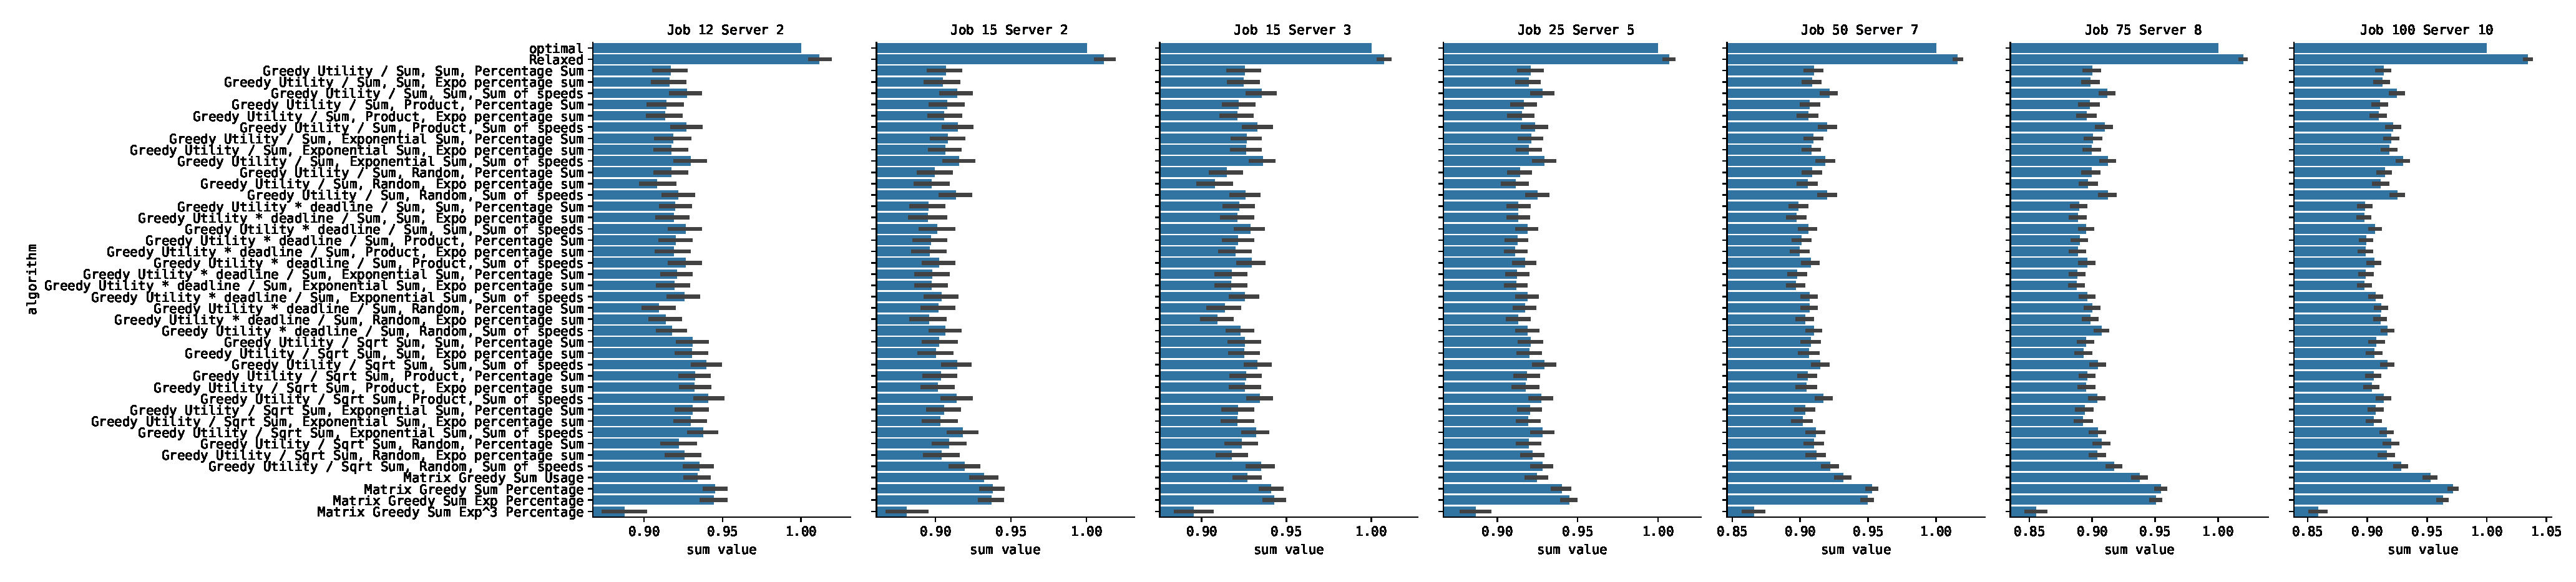
\includegraphics[width=\linewidth]{figures/greedy_big_small_sum_value.eps}
    \caption{Greedy algorithms with big small model measuring the sum of values}
\end{figure*}
\begin{figure*}
    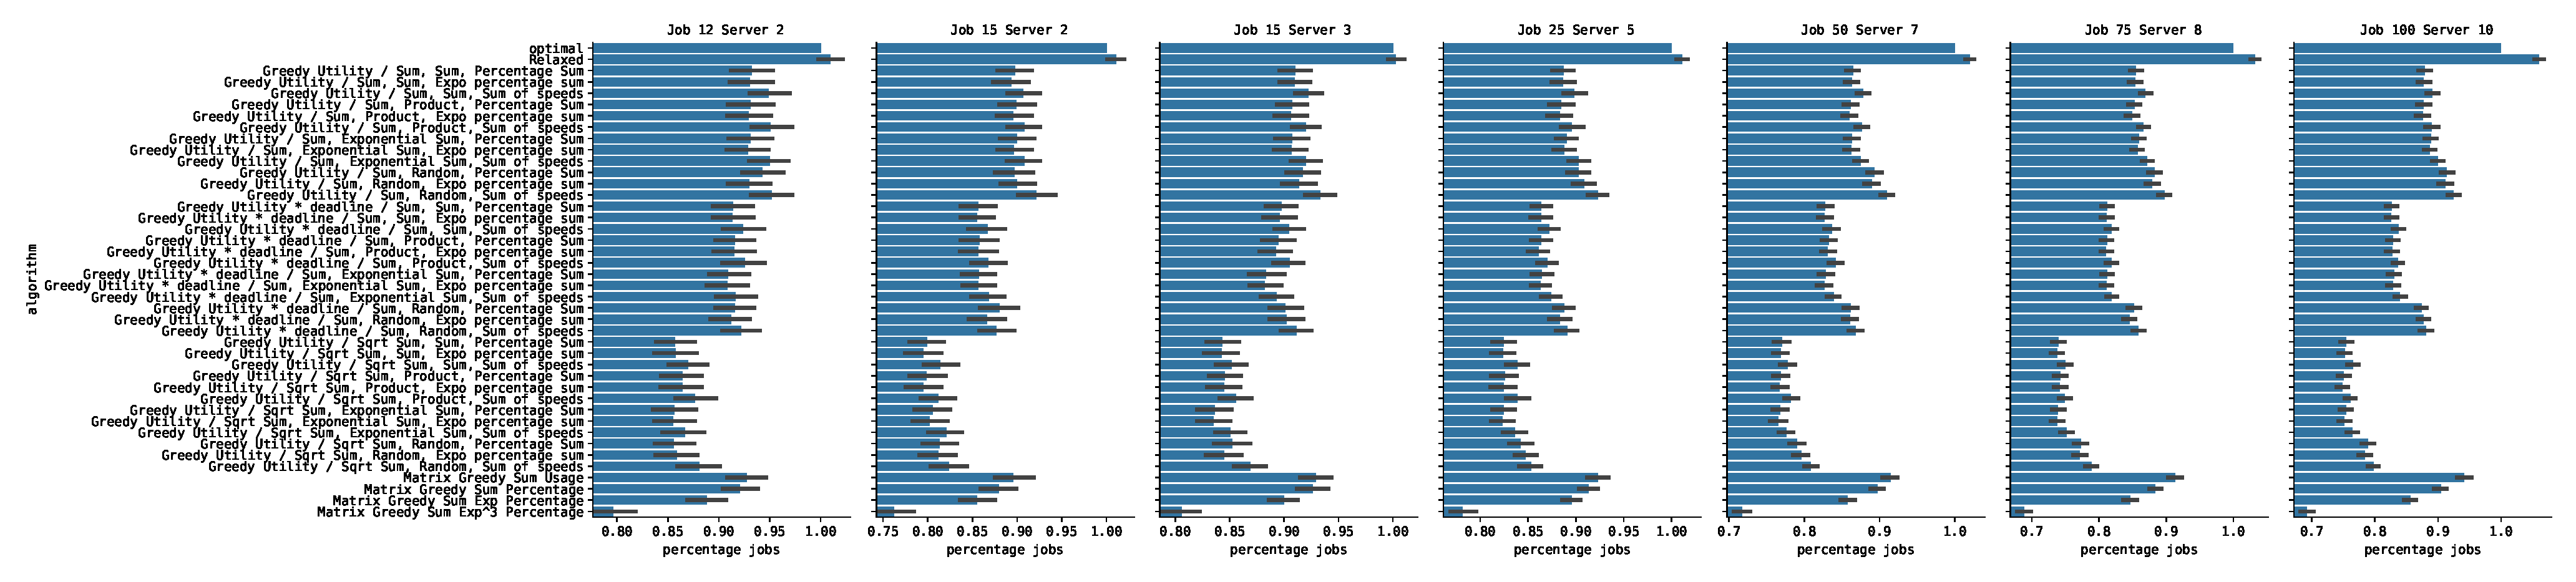
\includegraphics[width=\linewidth]{figures/greedy_big_small_percentage_jobs.eps}
    \caption{Greedy algorithms with big small model measuring the percentage of jobs allocated}
\end{figure*}

\begin{figure*}
    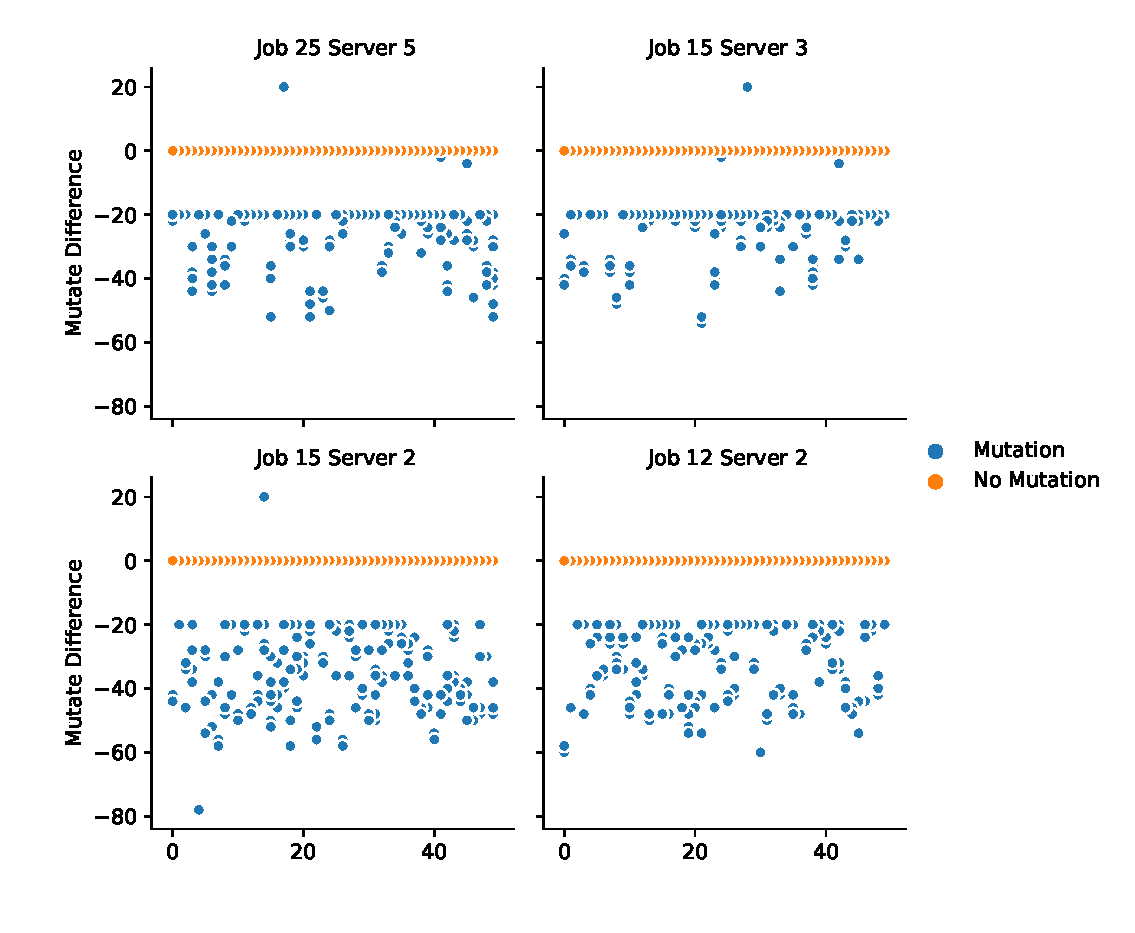
\includegraphics[width=\linewidth]{figures/job_mutation.eps}
    \caption{Measuring the difference in price when the job is incorrectly reported}
\end{figure*}
\begin{figure*}
    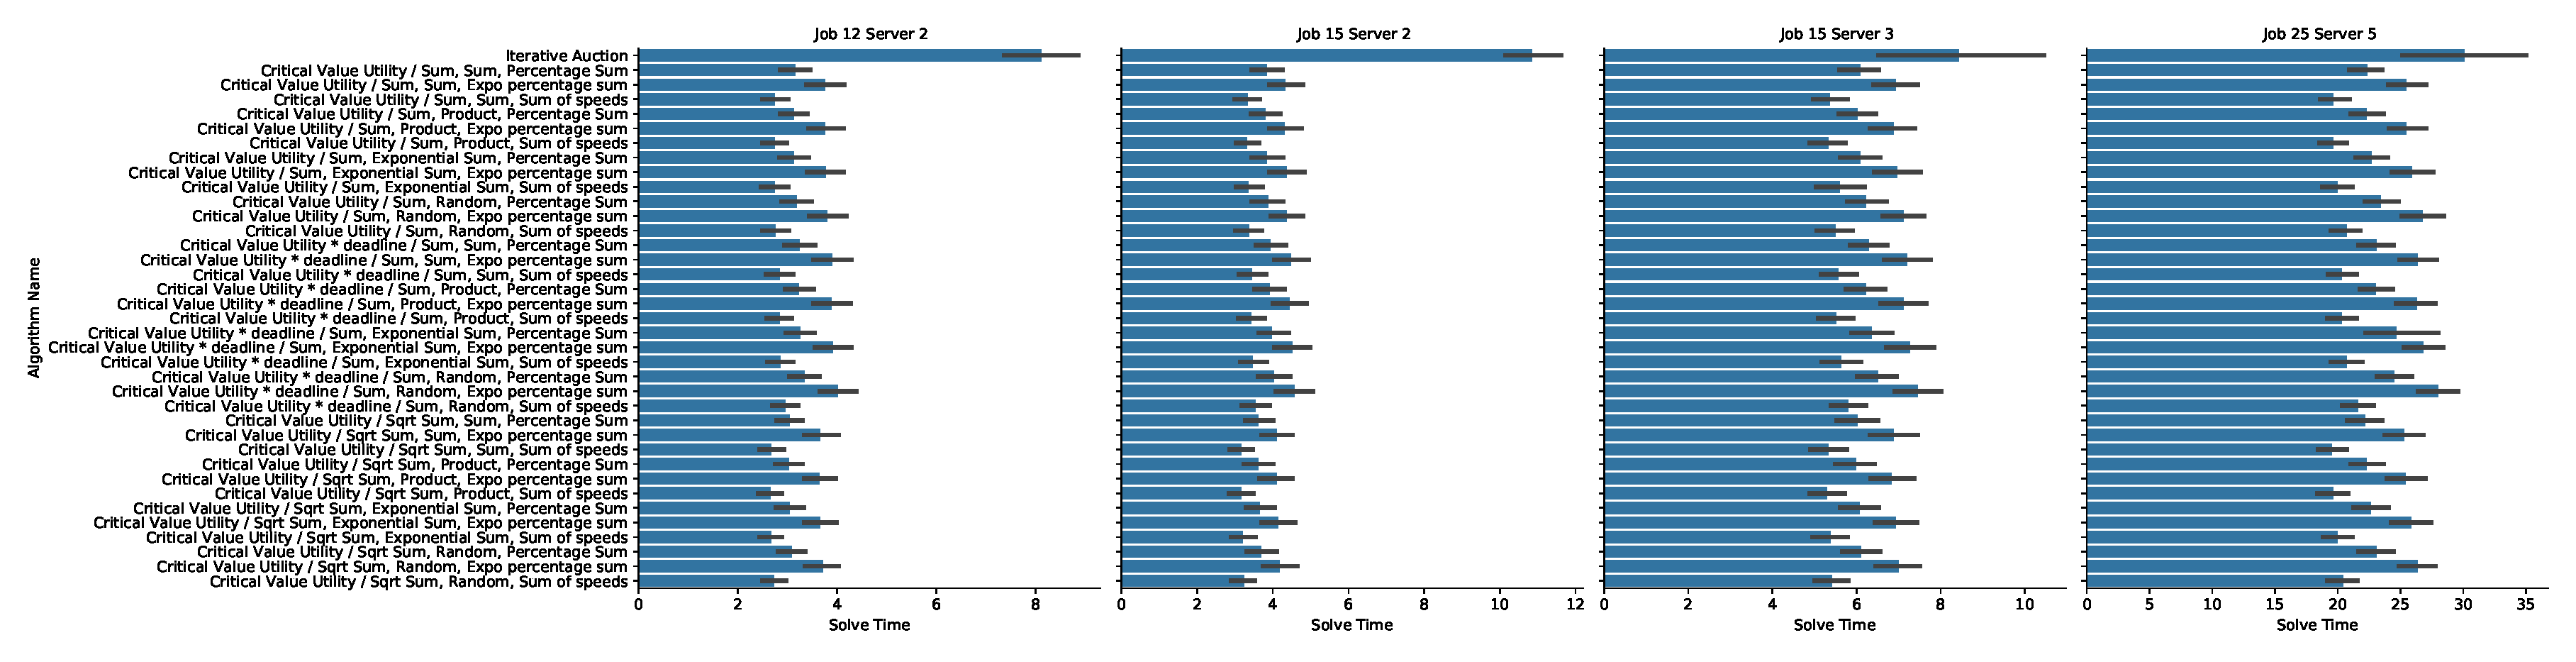
\includegraphics[width=\linewidth]{figures/critical_value.eps}
    \caption{The results from the critical value algorithm total price}
\end{figure*}

\begin{itemize}
    \item Greedy algorithms testing
    \item Job Mutations testing
    \item All possible job mutations testing
    \item Round number testing
    \item Uniform price change testing
    \item Non uniform price change testing
    \item Critical value pricing testing
\end{itemize}
\section{Conclusions and Future Work}
\begin{itemize}
    \item a
\end{itemize}

%%%%%%%%%%%%%%%%%%%%%%%%%%%%%%%%%%%%%%%%%%%%%%%%%%%%%%%%%%%%%%%%%%%%%%%%%%%%%%%%%%%%%%%%%%%%%%%%%%%%%%%%%
%% bibliography: see CFP for number of permitted pages

\bibliographystyle{ACM-Reference-Format}  % do not change this line!
\bibliography{bibliography}  % put name of your .bib file here

\end{document}
